\chapter{\textsc{Généralités}}
\section{\textsc{Moteur à combustion interne}}
\lettrine{E}{n} quelques mots, le moteur à combustion interne peut être defini comme un convertisseur de l'énergie chimique (la chaleur) contenue dans le fluide de travail en énergie mécanique ici recueilli dans le couple de l'arbre moteur.nous allons donc en distinguer deux sortes : moteur à apport de chaleur externe et moteur à combustion interne.\cite{sumuna}
\begin{figure}[h]
	\centering
	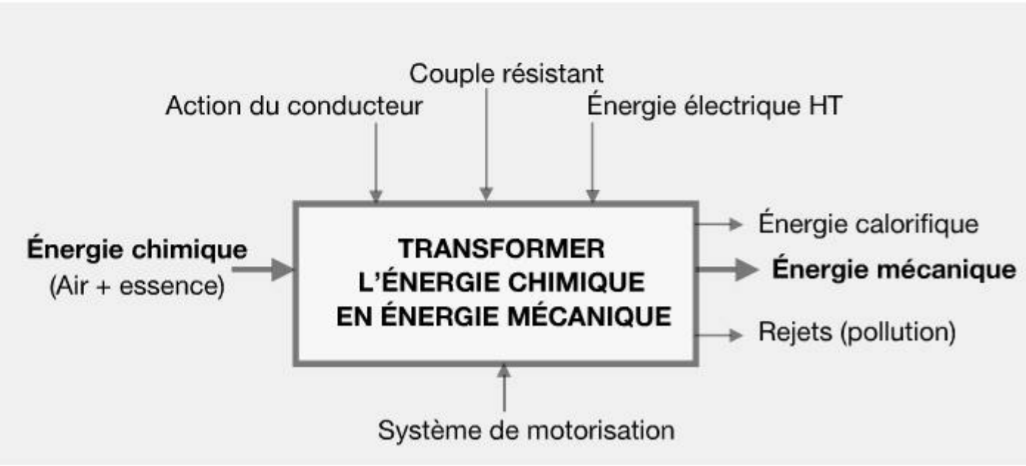
\includegraphics[width=0.7\linewidth]{Img/convertisseur}
	\caption[Convertisseur]{Convertisseur d'énergie thermique en mécanique}
	\label{fig:convertisseur}
\end{figure}

\subsection{Fonctionnement du moteur}
On distingue deux types des moteurs dans la famille de moteur à combustion interne :
\begin{itemize}
	\item Moteur à explosion (à essence) dans lequel la combustion du mélange aire - carburant est amorcée par l'étincelle une bougie d'allumage. Ils possèdent donc un système d'allumage commandé.\cite{tecauto}
	\item Moteur à combustion interne (Diesel) dont la combustion est déclenchée par l'injection des gaze sous pression dans de l'aire fortement comprimé. il se produit une auto - inflammation.\cite{tecauto}
\end{itemize}


Tous les moteurs à combustion interne à mouvement alternative se comporte de la même manière; on y trouve essentiellement les mêmes éléments (voir l'image \ref{fig:partie-du-moteur}) : La \textbf{Chambre de combustion} qui est un volume ou pénétré et réagissent les gaz; le \textbf{cylindre}, qui est le prolongement de la chambre de combustion; le \textbf{piston}, qui se déplace dans le cylindre et fais varier le volume de la chambre de combustion; le \textbf{Système bielle - manivelle}, qui est solidaire, à une extrémité, du piston et, à l’autre, du \textbf{vilebrequin}, et qui transforme le mouvement de va-et-vient du piston en un mouvement de rotation. le \textbf{bloc-moteur}, qui constitue l’enveloppe mécanique de l’ensemble.\cite{approche}


\begin{figure}[h]
	\centering
	\includegraphics[width=0.7\linewidth]{"Img/partie du moteur"}
	\caption[Partie du moteur]{Partie du moteur}
	\label{fig:partie-du-moteur}
\end{figure}
\begin{figure}[h]
	\centering
	\includegraphics[width=0.7\linewidth]{"Img/cycle theorique"}
	\caption[fonctionnement du moteur]{Fonctionnement du moteur}
	\label{fig:cycle-theorique}
\end{figure}


L'ingénieur français \emph{Beau de Rochas} a défini, en 1862, le principe du cycle de fonctionnement des moteurs à combustion interne dont les phases
sont :
%% Capsule historique note de marge___________________________
%%%%________________________________________________________

\begin{enumerate}
	\item Admission : aspiration d'air ou de mélange air-essence; 
	\item Compression du mélange air-carburant;
	\item Combustion et détente du piston;
	\item refoulement des gaz de combustion.
\end{enumerate} 
Il existe dans le monde trois types d'applications de ce cycle, dont vois-ci :
\begin{itemize}
	\item Moteur à quatre temps qui réalisent le cycle en quatre courses de piston et deux tours de vilebrequin;
	\item les moteurs à deux temps qui réalisent le cycle en deux courses de piston et un tour de vilebrequin;
	\item les moteurs rotatifs (walken) dont le mouvement rectiligne alternatif du piston classique est remplacé par la rotation d'un rotor qui réalise le cycle trois fois par tour.
\end{itemize}
Le fonctionnement théorique et réel du moteur est résumé dans l'image(\ref{fig:cycle-theorique}), permet de comprendre la situation analytique du rendement et les transmission des puissance.
\subsection{Rendement du moteur}
L'usage répandu du MCI dans diverses applications est dû à ses performances et à sa fiabilité.

\section{\textsc{Vue d'ensemble du système Segmentation-Piston-Chemise et état de l'art} }

\lettrine{L}{es} segments sont des anneaux brisés, de section carrée ou parallélépipédique, travaillant en extension. Ils doivent assurer des pressions radiales uniformes sur les parois du cylindre. La fonte douce qui les compose reçoit un chromage évitant une usure rapide par frottement. Leur position dans les gorges permet à la pression des gaz d'accentuer leur étanchéité.\cite{tecauto} Ils peuvent être au nombre de 2,3 ou 4 allant jusqu'à 5 sur les grands moteurs diesels suralimentés cala dépend du diamètre du piston. La fonction primaire de la segmentation c'est d'empêcher les fuites de gaz entre le piston et la chemise.Cependant, sans lubrification, ce contact étroit entre le segment et la chemise aurait comme conséquence de grandes pertes de puissance par frottement.En conséquence, l'autre objectif principal des segments est de distribuer efficacement le lubrifiant le long de l'interface segment/chemise, sans permettre à l'huile excessive de passer l'interface et de fuir vers la chambre de combustion où il pourrait être brulé.Une troisième fonction des segments qui est particulièrement importante pour le segment supérieur est la dissipation de la chaleur du piston vers le cylindre, comme montre la (figure \ref{fig:partie-du-segment}).\\

\begin{figure}
	\centering
	\includegraphics[width=0.7\linewidth]{"Img/partie du segment"}
	\caption[Segmentation]{Segmatation}
	\label{fig:partie-du-segment}
\end{figure}


Afin que ce système puisse atteindre efficacement ces objectifs globaux, chaque segment a un rôle unique. Le segment de dessus « coup de feu » scelle l'interface segment/chemise afin d'empêcher le gaz à haute pression de s'échapper de la chambre de combustion vers le carter (Blow by)\footnote{ }. Le segment \textbf{racleur} règle la quantité d'huile qui passe du carter pour lubrifier les segments supérieurs. Un deuxième segment est également présent dans la plupart des moteurs \textbf{segment d’étanchéité}, ce segment érafle en bas l'huile excessive qui passe l'interface segment racleur d'huile/chemise et vient en aide au premier segment affin de chasser le reste des gaz fuyards. La deuxième interface segment \textbf{d’étanchéité/chemise} fournit ainsi une barrière contre l'écoulement d'huile dans la gorge supérieure, et des gaz pour les parties plus inférieures du piston, ce qui réduit la consommation d’huile. \cite{ayad1}
\begin{figure}[h]
	\centering
	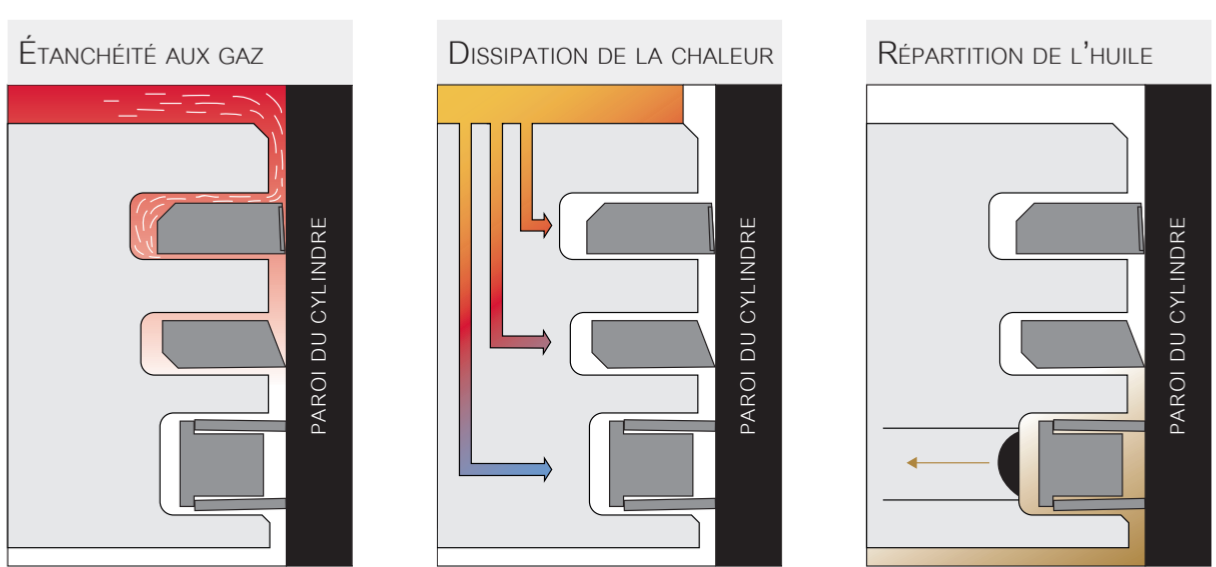
\includegraphics[width=0.7\linewidth]{Img/fonction-segment}
	\caption[Segments]{segments}
	\label{fig:fonction-segment}
\end{figure}
\\

L'interaction entre les segments et la chemise est décrit par le comportement tribologique le plus compliqué dans les moteurs à combustion interne.Lors du glissement du piston dans la chemise, le contact est soumis à des variations cycliques importantes et rapides de pression, de vitesse et de température.Cette variation a pour conséquence de faire balayer le contact segment-chemise par tous les régimes de lubrification. Les régimes de lubrification sont souvent illustrés par la courbe de Stribeck, illustrée dans la (figure \ref{fig:regime-de-lubrification}). Même si la courbe de Stribeck a été initialement développée pour les paliers lisses, elle est considérée comme applicable à d'autres systèmes lubrifiés.\cite{initiation} Car c'est une bonne représentation de la façon dont les régimes de lubrification dépendent de la vitesse, de la viscosité du lubrifiant et de la charge.

\begin{figure}[h]
	\centering
	\includegraphics[width=0.7\linewidth]{"Img/regime de lubrification"}
	\caption[Courbe de stribeck]{Regime de lubrification courbe de Stribeck}
	\label{fig:regime-de-lubrification}
\end{figure}



